% GNUPLOT: LaTeX picture with Postscript
\begingroup
  \makeatletter
  \providecommand\color[2][]{%
    \GenericError{(gnuplot) \space\space\space\@spaces}{%
      Package color not loaded in conjunction with
      terminal option `colourtext'%
    }{See the gnuplot documentation for explanation.%
    }{Either use 'blacktext' in gnuplot or load the package
      color.sty in LaTeX.}%
    \renewcommand\color[2][]{}%
  }%
  \providecommand\includegraphics[2][]{%
    \GenericError{(gnuplot) \space\space\space\@spaces}{%
      Package graphicx or graphics not loaded%
    }{See the gnuplot documentation for explanation.%
    }{The gnuplot epslatex terminal needs graphicx.sty or graphics.sty.}%
    \renewcommand\includegraphics[2][]{}%
  }%
  \providecommand\rotatebox[2]{#2}%
  \@ifundefined{ifGPcolor}{%
    \newif\ifGPcolor
    \GPcolortrue
  }{}%
  \@ifundefined{ifGPblacktext}{%
    \newif\ifGPblacktext
    \GPblacktexttrue
  }{}%
  % define a \g@addto@macro without @ in the name:
  \let\gplgaddtomacro\g@addto@macro
  % define empty templates for all commands taking text:
  \gdef\gplbacktext{}%
  \gdef\gplfronttext{}%
  \makeatother
  \ifGPblacktext
    % no textcolor at all
    \def\colorrgb#1{}%
    \def\colorgray#1{}%
  \else
    % gray or color?
    \ifGPcolor
      \def\colorrgb#1{\color[rgb]{#1}}%
      \def\colorgray#1{\color[gray]{#1}}%
      \expandafter\def\csname LTw\endcsname{\color{white}}%
      \expandafter\def\csname LTb\endcsname{\color{black}}%
      \expandafter\def\csname LTa\endcsname{\color{black}}%
      \expandafter\def\csname LT0\endcsname{\color[rgb]{1,0,0}}%
      \expandafter\def\csname LT1\endcsname{\color[rgb]{0,1,0}}%
      \expandafter\def\csname LT2\endcsname{\color[rgb]{0,0,1}}%
      \expandafter\def\csname LT3\endcsname{\color[rgb]{1,0,1}}%
      \expandafter\def\csname LT4\endcsname{\color[rgb]{0,1,1}}%
      \expandafter\def\csname LT5\endcsname{\color[rgb]{1,1,0}}%
      \expandafter\def\csname LT6\endcsname{\color[rgb]{0,0,0}}%
      \expandafter\def\csname LT7\endcsname{\color[rgb]{1,0.3,0}}%
      \expandafter\def\csname LT8\endcsname{\color[rgb]{0.5,0.5,0.5}}%
    \else
      % gray
      \def\colorrgb#1{\color{black}}%
      \def\colorgray#1{\color[gray]{#1}}%
      \expandafter\def\csname LTw\endcsname{\color{white}}%
      \expandafter\def\csname LTb\endcsname{\color{black}}%
      \expandafter\def\csname LTa\endcsname{\color{black}}%
      \expandafter\def\csname LT0\endcsname{\color{black}}%
      \expandafter\def\csname LT1\endcsname{\color{black}}%
      \expandafter\def\csname LT2\endcsname{\color{black}}%
      \expandafter\def\csname LT3\endcsname{\color{black}}%
      \expandafter\def\csname LT4\endcsname{\color{black}}%
      \expandafter\def\csname LT5\endcsname{\color{black}}%
      \expandafter\def\csname LT6\endcsname{\color{black}}%
      \expandafter\def\csname LT7\endcsname{\color{black}}%
      \expandafter\def\csname LT8\endcsname{\color{black}}%
    \fi
  \fi
  \setlength{\unitlength}{0.0500bp}%
  \begin{picture}(7200.00,5040.00)%
    \gplgaddtomacro\gplbacktext{%
      \csname LTb\endcsname%
      \put(942,1289){\makebox(0,0){\strut{}-5}}%
      \csname LTb\endcsname%
      \put(1266,1230){\makebox(0,0){\strut{}-4}}%
      \csname LTb\endcsname%
      \put(1590,1170){\makebox(0,0){\strut{}-3}}%
      \csname LTb\endcsname%
      \put(1914,1111){\makebox(0,0){\strut{}-2}}%
      \csname LTb\endcsname%
      \put(2238,1051){\makebox(0,0){\strut{}-1}}%
      \csname LTb\endcsname%
      \put(2562,992){\makebox(0,0){\strut{} 0}}%
      \csname LTb\endcsname%
      \put(2886,933){\makebox(0,0){\strut{} 1}}%
      \csname LTb\endcsname%
      \put(3209,873){\makebox(0,0){\strut{} 2}}%
      \csname LTb\endcsname%
      \put(3533,814){\makebox(0,0){\strut{} 3}}%
      \csname LTb\endcsname%
      \put(3856,754){\makebox(0,0){\strut{} 4}}%
      \csname LTb\endcsname%
      \put(4180,695){\makebox(0,0){\strut{} 5}}%
      \csname LTb\endcsname%
      \put(4398,755){\makebox(0,0){\strut{}-8}}%
      \csname LTb\endcsname%
      \put(4632,884){\makebox(0,0){\strut{}-6}}%
      \csname LTb\endcsname%
      \put(4866,1013){\makebox(0,0){\strut{}-4}}%
      \csname LTb\endcsname%
      \put(5100,1141){\makebox(0,0){\strut{}-2}}%
      \csname LTb\endcsname%
      \put(5333,1270){\makebox(0,0){\strut{} 0}}%
      \csname LTb\endcsname%
      \put(5567,1398){\makebox(0,0){\strut{} 2}}%
      \csname LTb\endcsname%
      \put(5801,1527){\makebox(0,0){\strut{} 4}}%
      \csname LTb\endcsname%
      \put(6035,1656){\makebox(0,0){\strut{} 6}}%
      \csname LTb\endcsname%
      \put(6268,1784){\makebox(0,0){\strut{} 8}}%
      \put(920,1384){\makebox(0,0)[r]{\strut{} 0}}%
      \put(920,1613){\makebox(0,0)[r]{\strut{} 0.1}}%
      \put(920,1842){\makebox(0,0)[r]{\strut{} 0.2}}%
      \put(920,2070){\makebox(0,0)[r]{\strut{} 0.3}}%
      \put(920,2299){\makebox(0,0)[r]{\strut{} 0.4}}%
      \put(920,2527){\makebox(0,0)[r]{\strut{} 0.5}}%
      \put(920,2755){\makebox(0,0)[r]{\strut{} 0.6}}%
      \put(920,2984){\makebox(0,0)[r]{\strut{} 0.7}}%
      \put(920,3212){\makebox(0,0)[r]{\strut{} 0.8}}%
      \put(920,3441){\makebox(0,0)[r]{\strut{} 0.9}}%
      \put(188,2413){\makebox(0,0){\strut{}$\omega_i$}}%
    }%
    \gplgaddtomacro\gplfronttext{%
      \csname LTb\endcsname%
      \put(2264,677){\makebox(0,0){\strut{}$\gamma_i^1$}}%
      \put(6029,1156){\makebox(0,0){\strut{}$\gamma_i^2$}}%
      \put(188,2413){\makebox(0,0){\strut{}$\omega_i$}}%
    }%
    \gplbacktext
    \put(0,0){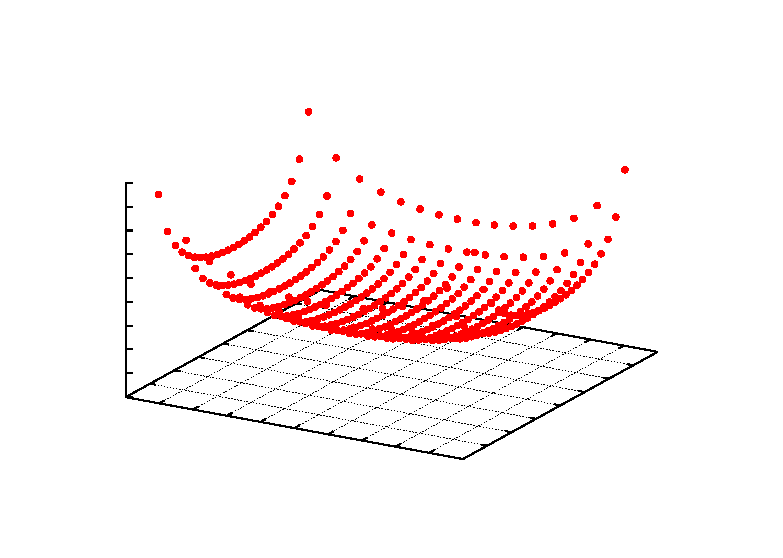
\includegraphics{tp-rule}}%
    \gplfronttext
  \end{picture}%
\endgroup
